\section{Introduction to Reinforcement Learning}
\textit{This section reviews the lecture slides 1 and 2 (until Monte Carlo). }
\begin{itemize}
	\item Reinforcement Learning deals with the following question: 
	
	How to \textcolor{blue}{sequentially interact} with an environment to \textcolor{blue}{maximize a long-term objective}?
	
	\item The general RL setting is visualized in Figure~\ref{fig:rl_introduction_reinforcement_learning}. Thereby we have 4 variables that are passed around:
	\begin{itemize}
		\item The state $S_t$, in which the agent currently is, determined by the environment
		\item The action $A_t$ which is chosen by the agent, based on the observation of the state $S_t$
		\item Based on the interaction $A_t$, the agent ends up in a new state $S_{t+1}$ as well as getting a reward $R_{t+1}$. Both properties are determined by the environment, and can only be influenced by the agent through $A_t$
	\end{itemize}
	\begin{figure}[ht!]
		\centering
		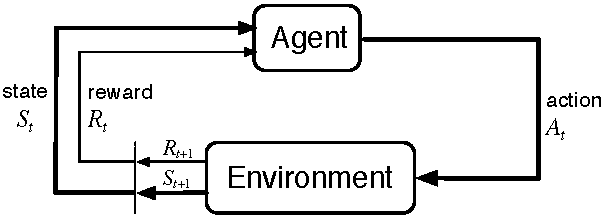
\includegraphics[width=0.4\textwidth]{figures/rl_introduction_reinforcement_learning.pdf}
		\caption{Illustration of the interaction of an agent with an environment in the reinforcement learning setting.}
		\label{fig:rl_introduction_reinforcement_learning}
	\end{figure}

	\item The decision of which action to take at which state is called policy, and we denote it by $\pi$. The goal is to find the optimal policy $\pi$ which maximizes the reward we get from the environment
		
	\item As we learn by interactions, we have major main challenges in contrast to standard supervised learning:
	\begin{itemize}
		\item The dataset is not static as in e.g. image classification. Every time we change our policy, new data has to be generated as the actions we take at certain states are different. Note that there are techniques to use the data more efficiently, and we will discuss them later.  
		\item Instead of having i.i.d. data, we have sequential data which are highly correlated. Standard optimizers like SGD fail because they assume i.i.d. inside a batch. We will also discuss how we can tackle this problem.
	\end{itemize}
\end{itemize}
\subsection{MDPs and $k$-armed bandits}
\begin{itemize}
	\item A common used, simplified example for RL is a $k$-armed bandit. We can image it as $k$ slot machines with unknown pay-off distribution. Hence, we have a static environment where the mapping function between actions and rewards is independent of state and time step $t$
	\item Our goal is to maximize the cumulative reward over time. There are two variants we can use:
	\begin{itemize}
		\item If we want to maximize our reward for a finite horizon $T$ (i.e. limited number of trials), our goal is to maximize $\sum_{t=1}^{T} r_t$
		\item If we assume that we can take as many actions as we want, we have the objective for infinite horizon: $\sum_{t=1}^{\infty} \gamma^{t}r_t$ where $\gamma\in [0,1]$ is a discount factor. Note that if we would not have a discount factor, we end up with infinite reward for any action whose reward has a mean greater than zero.
		\item For generalization, we call $G_t=\sum_{k=0}^{\infty} \gamma^{k}R_{t+k+1}=R_{t+1}+\gamma G_{t+1}$ the \textbf{(discounted) return}, or cumulative reward, at time step $t$. Only if a episode terminates (meaning that we cannot play forever), a discount factor of $\gamma=1$ is allowed.
	\end{itemize} 
	\item A general trade-off in reinforcement learning is between \textbf{exploration} (i.e. trying new actions) and \textbf{exploitation} (i.e. taking best actions we know). If we perform too little exploration, we might overlook the best action, for example due to stochasticity of the reward. However, exploiting the best actions is likely to lead to the maximum rewards, so that with exploring, we ``lose'' possible rewards.
	
	A general rule of thumb is: if we have much time left or are very uncertain about our current estimates, do more exploration. If we are limited on time, or are certain about our estimates, we should exploit more. 
	
	Also $\gamma$ can play a role as the higher $\gamma$, the more we care about rewards in the future, and hence, should perform more exploration.
	
	\item We now introduce a set of important functions which are used for finding the optimal policy:
	\begin{itemize}
		\item The \textbf{state-action value function}, also called \underline{$q$-function}, expresses the expected return of taking a certain action in a given state:
		$$q_{\pi}(s,a)=\E_{\pi}[G_t|S_t=s,A_t=a]$$
		Note that $q$-value is always specific to a certain policy as $G_t$ is in expectation that all steps after $t$ are taken according to the policy $\pi$
		\item The \textbf{state-value function} is similar to the $q$ function, but only takes the state into account, and considers the action under the expectation:
		$$v_{^\pi}(s)=\E_{\pi}[G_t|S_t=s]$$
	\end{itemize}

	\item In the case of the k-armed bandit, we try to learn a $q$-function (as we want to find the best action) but assume that we stay in the same state $s$. To balance exploration and exploitation, there are different strategies possible, for example:
	\begin{itemize}
		\item \textbf{$\epsilon$-greedy} takes in $(1-\epsilon)$ cases the optimal action, and with the chance of $\epsilon$ selects an action randomly
		\item An annealed softmax takes the estimated action value into account, and creates a distriubtion based on this with a temperature factor $\tau$ (high $\tau$ means more stochasticity):
		$$p(a)=\frac{\exp\left(\hat{q}(a)/\tau\right)}{\sum_{a'}\exp\left(\hat{q}(a')/\tau\right)}$$
		\item We can use the current estimate $\hat{q}$ in combination with the uncertainty we have a certain action. This leads to the Upper confidence bound, or we can alternatively initialize all $q$-values optimistically (guarantees certain level of exploration)
	\end{itemize} 

	\item \textbf{Markov Decision Process}: An agent chooses an action which only depends on the current state $s_t$, and is independent of the history $s_0,...,s_{t-1}$ given $s_t$. Formally, we can define a finite MDP by
	\begin{itemize}
		\item A finite set of states $\mathcal{S}$
		\item A finite set of actions for each state $\mathcal{A}_s$ (often the same in all states)
		\item A dynamics function $p(s',r|s,a)=\Prob{S_t=s',R_t=r|S_{t-1}=s,A_{t-1}=a}$ which is often split into
		\begin{itemize}
			\item Transition function $p(s'|s,a)$
			\item Reward function $p(r|s,a,s')$
		\end{itemize}
		\item A discount factor $\gamma\in[0,1]$
	\end{itemize}
	\item In this setting, the optimal action can be found by optimizing the policy $\pi^{*}(s_t)$. In the rest of the course, we mostly focus on MDPs
\end{itemize}

\subsection{Dynamic Programming}
\begin{itemize}
	\item For simple environments where we know the dynamics function of the MDP, we can apply approaches of dynamic programming
	\item One thing to notice about the functions $v$ and $q$ are their relationships, namely:
	\begin{equation*}
		\begin{split}
			v(s) & = \E_{\pi}\left[G_t|S_t=s\right] = \E_{a\sim\pi}\left[\E_{\pi}\left[G_t|S_t=s,A_t=a\right]\right] = \E_{a\sim\pi} q_{\pi}(s,a)\\[8pt]
			q(s,a) & = \E_{\pi}[G_t|S_t=s,A_t=a] = \E_{\pi}[R_{t+1}|S_t=s,A_t=a]+\E_{s',\pi}[\gamma G_{t+1}|S_{t+1}=s'] \\& = \E_{s',\pi}[R_{t+1}+\gamma v(s')|S_t=s,A_t=a,S_{t+1}=s']
		\end{split}
	\end{equation*}
	\item A policy is optimal if there is no other policy for which the value of any state is larger than the current one: $v_{*}(s)=\max_{\pi} v_{\pi}(s)$, $q_{*}(s,a)=\max_{\pi} q_{\pi}(s,a)$
	\item Again, we can write down the relations between the two functions, which are called \textit{Bellman optimality equations} for the optimal case:
	\begin{equation*}
		\begin{split}
			v_{*}(s) & =\max_{a}q_{*}(s,a)= \max_a \E\left[R_{t+1}+\gamma v_{*}(S_{t+1})|S_t=s,A_t=a\right]\\
			q_{*}(s,a) & = \E\left[R_{t+1}+\gamma \max_{a'} q_{*}(S_{t+1},a')\Big\vert S_t=s,A_t=a\right]
		\end{split}
	\end{equation*}
	
	\item The first approach of finding the optimal policy is \textbf{policy iteration}. It combines two steps:
	\begin{itemize}
		\item \textit{Policy evaluation}: given a policy $\pi$, we try to find the corresponding value function $v_{\pi}$. We do this by performing the update $v(s)=\E[R_{t+1}+\gamma v(s)]$ until the values converge. Note that we can evaluate the expectation as we know $\pi$ and the MDP dynamics $p(s',r|s,a)$
		\item \textit{Policy improvement}: given the value function $v_{\pi}$, we try to find a new policy for which we know that $\forall s, v_{\pi'}(s)\geq v_{\pi}(s)$. We can do that by taking the argmax over actions in each state.
	\end{itemize}
	Policy iteration performs these two in a loop until the policy is not changed anymore in the improvement step. It is guaranteed to converge to the optimal policy $\pi$.
	
	The full algorithm is shown in Figure~\ref{fig:rl_introduction_policy_iteration}.
	\begin{figure}[ht!]
		\centering
		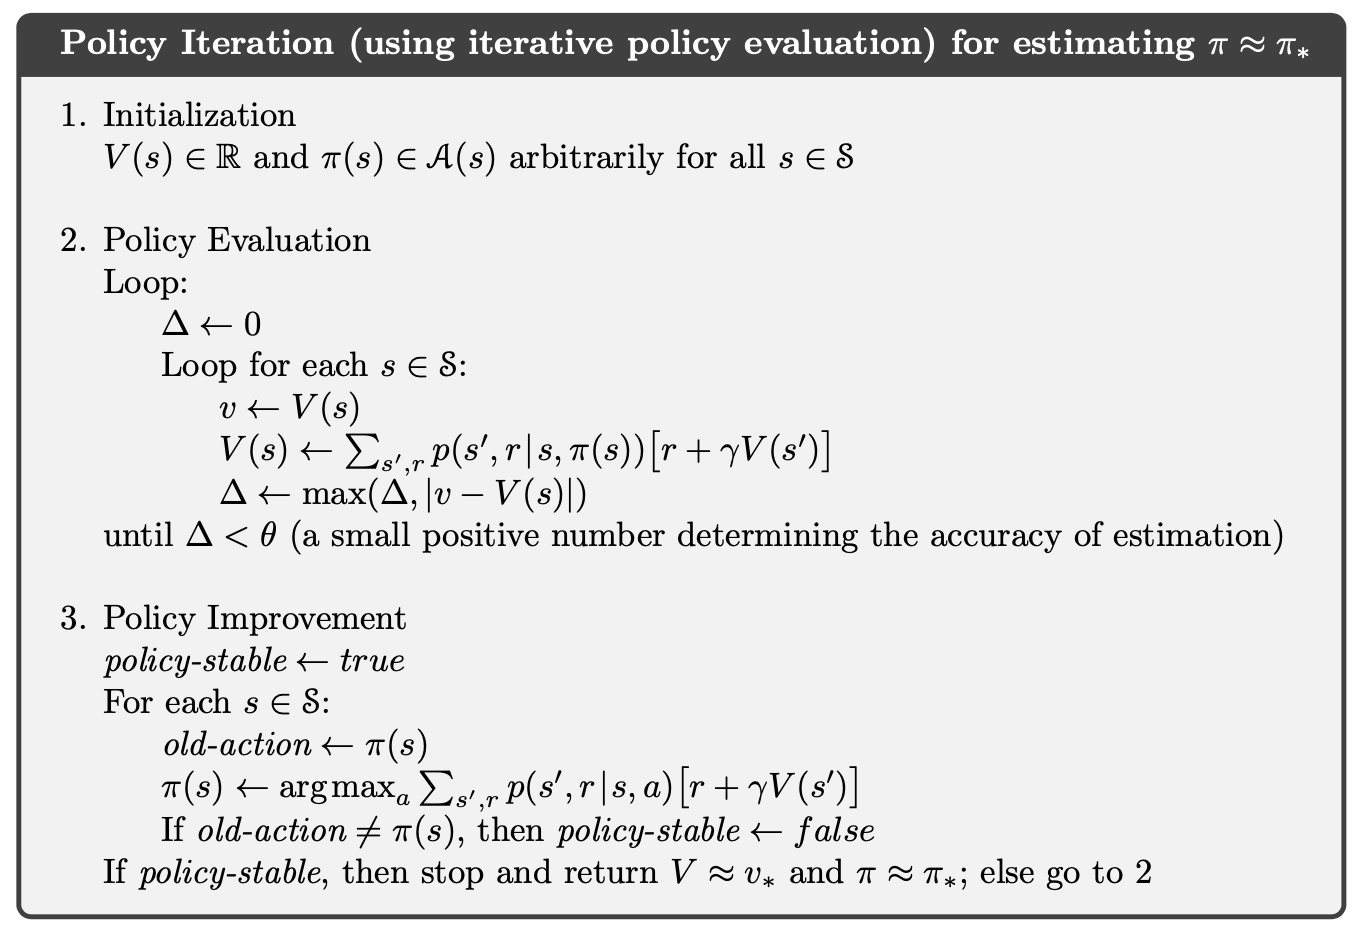
\includegraphics[width=0.7\textwidth]{figures/rl_introduction_policy_iteration.png}
		\caption{Policy iteration algorithm (Sutton book)}
		\label{fig:rl_introduction_policy_iteration}
	\end{figure}
	\item The issue of policy iteration is that the policy evaluation step can take a long time until it fully converges, although slight changes might not influence the policy too much. An alternative is to stop policy evaluation after a single iteration, and directly optimize it. This leads to the \textbf{value iteration algorithm}.
	
	When implementing it, we can efficiently combine the two steps of evaluation and improvement, which is actually the same as performing the Bellman optimality equation as an update step. See Figure~\ref{fig:rl_introduction_value_iteration} for details.
	
	\begin{figure}[ht!]
		\centering
		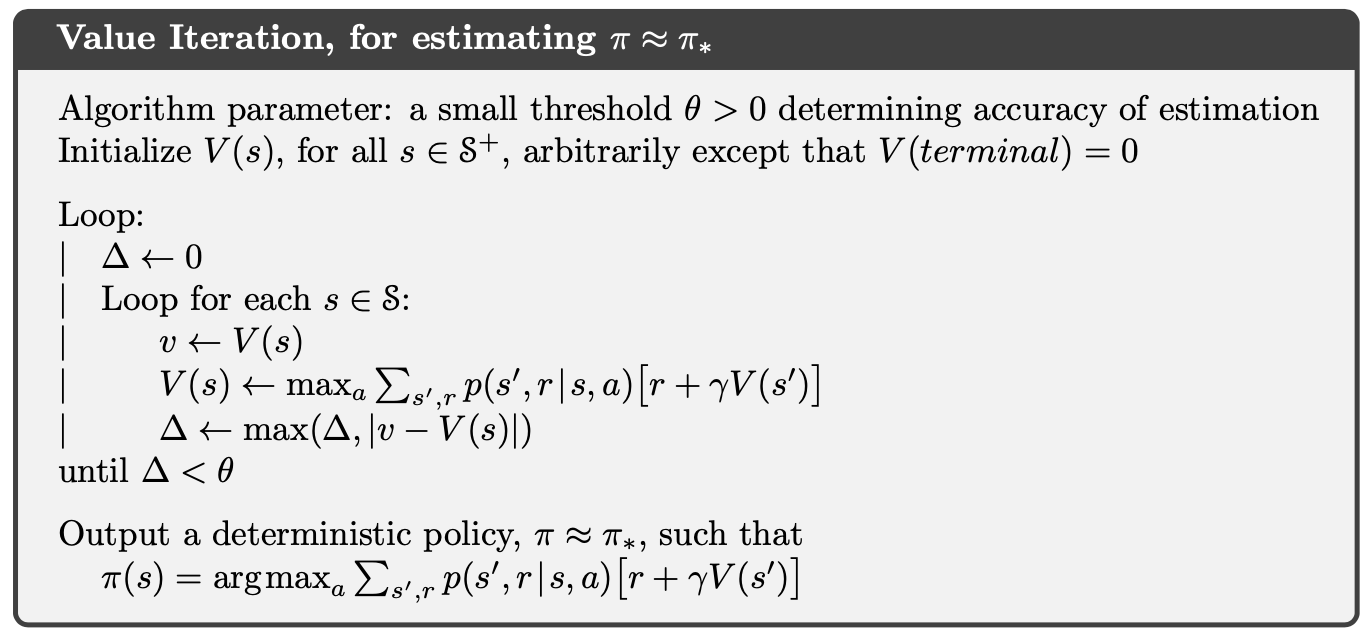
\includegraphics[width=0.7\textwidth]{figures/rl_introduction_value_iteration.png}
		\caption{Value iteration algorithm (Sutton book)}
		\label{fig:rl_introduction_value_iteration}
	\end{figure}

	The drawback of value iteration is that it can lead to noisy updates as it only performs a single update step and hence, can give inaccurate estimates of $v$. In practice, what has been found to mostly work the best, is to perform a limited, small number of steps of policy evaluation.
	
	\item Keep in mind that for all these algorithms we require to know the MDP dynamics $p(s',r|s,a)$. However, this is often not the case, especially for more complicated, real-world environments. There we can only sample data point $(s_i,a_i,r_i,s'_i)$ which we need to use effectively. 
	
\end{itemize}
\subsection{Outline}
\begin{itemize}
	\item In the next sections (and rest of the whole course), we will deal with different ways of learning the optimal policy when the dynamics of the MDP are unknown in advance. We can distinguish the approaches into three main groups (see Figure~\ref{fig:rl_introduction_overview_leanring_techniques}):
	\begin{itemize}
		\item \textbf{Value-based} methods try to learn the value functions $v(s)$ and $q(s,a)$ from interactions with the environment. Based on these, we can find the optimal policy $\pi$.
		\item \textbf{Policy-based} methods try to directly learn the desired objective, namely the policy $\pi$. While we prevent propagating errors to the policy from learning a value function, it is often harder to optimize.
		\item In contrast to the previous techniques, \textbf{model-based} RL is based on the idea of learning the dynamics of the MDP, namely $p(s',r|s,a)$. With this knowledge given, we can then again apply value-based or policy-based methods, but support them by either using the transition function directly (i.e. take all possible future states into account instead of sampling), or simulate new trajectories if this is expensive in the original environment. 
	\end{itemize}
	\begin{figure}[ht!]
		\centering
		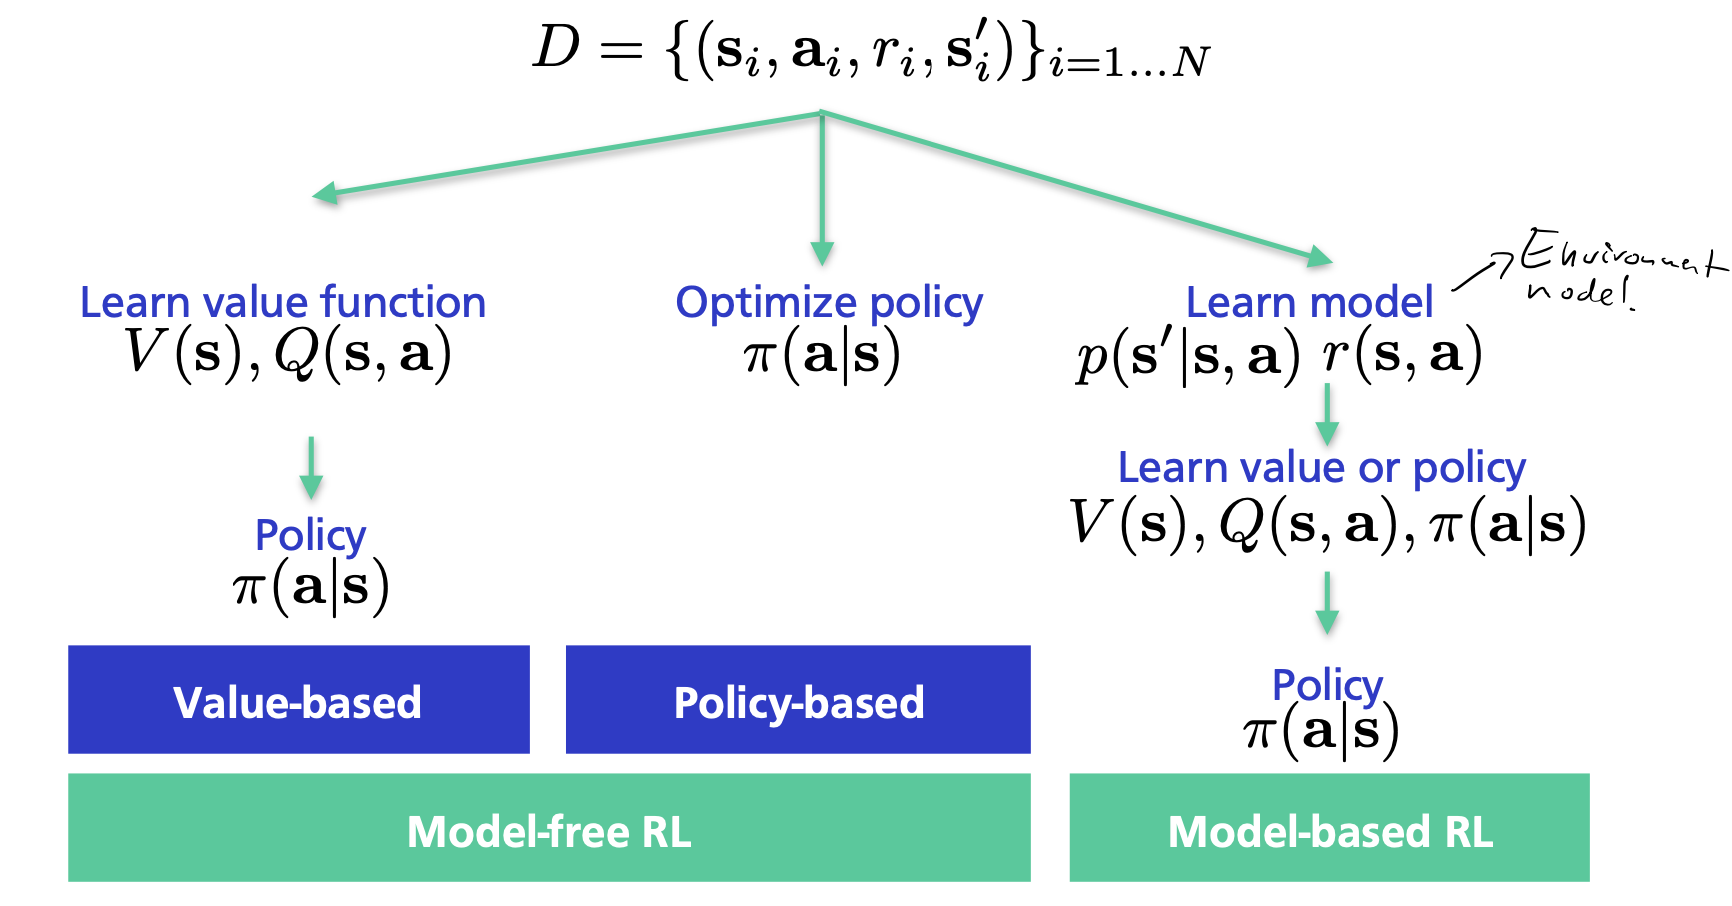
\includegraphics[width=0.5\textwidth]{figures/rl_introduction_overview_leanring_techniques.png}
		\caption{Overview of different learning strategies in RL.}
		\label{fig:rl_introduction_overview_leanring_techniques}
	\end{figure}
	\item The next sections 2 and 3 (lecture slides 3 to 6) deal with value-based methods. First, we discuss tabular-based techniques, meaning that we store e.g. $v(s)$ by a big table (i.e. every state has an entry in this table). However, these methods cannot be applied if the state space is continuous and/or high-dimensional (size increases exponentially). Thus, we look at approximations in section 3.
	\item Section 4 (lecture slides 7 to 10) deals with policy-based RL introducing different techniques for approximating the optimal gradients in policy learning.
	\item Model-based RL is discussed in section 5 (lecture slides 11 and 12), but in less details than the previous two.
	\item The final chapter deals with partially-observable environments (Section 7, lecture 13), and how to take uncertainty into account.
\end{itemize}